\chapter{Results}
This chapter describes how your results answer your research question. The results obtained are related back to the research question (and possibly the hypothesis), giving consideration also to the information found during the secondary research, and findings are determined.

\section{Implementation based results}
If your project was based on writing software, you will need to demonstrate how your working system can be used to answer your research question.

\section{Empirical investigations}
If your project was based on collecting data, you will need to demonstrate how your data corroborates or disproves your hypothesis. Where the findings are based on subjective evidence, as in the case of study project, a validation exercise is required. Here the findings are subjected to scrutiny, either by experts, or perhaps by applying them to a real-world situation to determine how well they stand up. In either case the findings are often refined as a result. (Where the findings arise from evidence obtained rigorously from a representative sample, validation is not required.)

\section{Presenting results}
You will often need to present results as a figure, such as Figure 5.1. Note how the figure numbers are automatically generated by Word.

\begin{figure}[h]
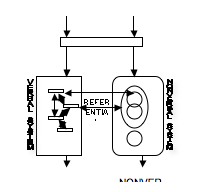
\includegraphics	{diagram2.png}
\caption{Paivio's Dual coding Framework}
\end{figure}

Tables, such as Table 5.1 and Table 5.2 Data requirements for Study 1 can also be a good way of presenting data. Note that Figures and Tables are both automatically inserted into the tables of contents.

\begin{table}[h]
	\begin{tabular}{| p{3.6cm} | p{3.6cm} | p{3.6cm} |}
	\hline
	Artefacts & 
	\begin{itemize*}
	\item[] Photographs
	\item[] Drawings
	\item[] Maps
	\item[] Diagrams
	\item[] Graphs
	\end{itemize*}
 & 
	\begin{itemize*}
	\item[] Natural human languages
	\item[] Formal systems (Fregian) such as
	\item[] Mathematics
	\item[] Symbolic logic
	\item[] Computer languages
	\end{itemize*}
 \\ \hline
 	Properties &
	\begin{itemize*}
		\item[] Analogue
		\item[] Iconic
		\item[] Continuous
		\item[] Referentially isomorphic (has links to other representations)
	\end{itemize*}
	& 
	\begin{itemize*}
		\item[] Non-analogue
		\item[] Non-iconic
		\item[] Digital or discrete (as opposed to continuous)
		\item[] Referentially arbitrary (does not have links to other representations)
		\item[] Propositional 
	\end{itemize*}
	\\ \hline
	\end{tabular}
\caption{Characteristics of Paivio's picture-like and language-like dimensions}
\end{table}

\begin{table}[h]
	\begin{tabular}{ | p{1cm} | p{4.6cm} | p{2cm} | p{4.6cm} | }
	\hline
	Approach & Research Questions & Group &  Data Requirements \\
	\hline
	1 & What are the preferences and perceptions of different representations in the CS domain? & Student
and
Academic
 & Information that reveals perspectives and preferences in representation and more implicit knowledge about these preferences and perspectives \\
	\hline
	2 & What are the individual differences in learning? & Student
and
Academic
 & Inventory measures of individuals’ preferences and tendencies in learning \\
	\hline
	3 & What are the individual background factors that might have an impact on preferences and perceptions in representation? & Student
and
Academic
 & Individual background information about learners and academics such as age, gender, prior experience, etc. \\
	\hline
	4 & If any incidental learning has taken place can it be attributed to a particular representation? & Student & Pre- and post-test scores of simple recall of information that reveal any improvements in learning as a result of being exposed to particular representations \\
	\hline
	5 & What criteria do academics use for choosing representations in instructional materials? & Academic & Information about criteria that individual academics have used in relation to instructional materials that they have produced \\
	\hline
	\end{tabular}
	\caption{Data requirements for Study 1}
\end{table}

\section{Validation}
Whatever form of research you carried out, you should consider how your initial research question has been shown to be answered/not answered/in need of modification.

\subsection{Analysis}
You may wish to consider how your choices of method, implementation and data have affected your research, and whether different choices (for future work, perhaps) might have found better results.
